\subsection{KNN Results}

For each movie, one of five CPU usage sequences is selected as query sequence and the rest four sequences are considered database (training) sequences, as described in \ref{sec:experimental_setup}, 
Then both query sequences and database sequences are divided into query subsequences and database subsequences with the same length.
For sequences with 1-second intervals, the length of subsequeces $l$ is set to $l = [60, 120, 180, 300, 600]$, and each subsequence is extracted at every 20-second interval. 
For sequences with 5-second intervals, the length of subsequences $l$ is set to $l = [60, 120, 180, 300]$, and each subsequence is extracted at every 5-second interval. 

After building up query subsequences and database subsequences, we apply KNN method in order to classify each query subsequence based on database subsequences and predict the movie title of each subsequence. 
In this experiment, $k$ value is set to 3 since the maximum number of correct neighbors is 4. 
The accuracy of classification according to the length of subsequence is shown in Figure \ref{fig:experiment_knn}.
The accuracy is low as 46$\%$ when subsequence length is set to 60-second.
However, the accuracy increases up to 88$\%$ when subsequence is set to 180-second.
The experimental result shows that given 10 movies and CPU usage statistics of 150 seconds, our side channel attack correctly predicts which movie a user is watching at the accuracy of higher than 80$\%$.

\begin{table}[h!]
\begin{center}
\begin{tabular}{|c||c|c|c|c|c|c|c|c|c|c|}
\hline
\multirow{2}{*}{Movie ID} & \multicolumn{5}{c|}{Prediction Precision}	\\
\cline{2-6}
	& 60 & 120 & 180 & 300 & 600		\\
\hline
1	& 0.18	& 0.30	& 0.37	& 0.42	& 0.62		\\
2 	& 0.57	& 0.64	& 0.73	& 0.94	& 1.00		\\
3 	& 0.51	& 0.56	& 0.64	& 0.75	& 0.91		\\
4	& 0.53	& 0.67	& 0.79	& 0.93	& 1.00		\\
5	& 0.81	& 0.93	& 0.97	& 0.95	& 0.99		\\
6	& 0.83	& 0.95	& 0.97	& 0.98	& 1.00		\\
7 	& 0.27	& 0.30	& 0.38	& 0.46	& 0.58		\\
8 	& 0.66	& 0.84	& 0.89	& 0.99	& 1.00		\\
9 	& 0.54	& 0.77	& 0.89	& 0.97	& 0.99		\\
10 	& 0.50	& 0.79	& 0.91	& 0.95	& 1.00		\\	
\hline
\hline
Overall & 0.54	& 0.68	& 0.77	& 0.83	& 0.91	 	\\
\hline
\end{tabular}
\end{center}
\caption{Success Rate of Prediction - KNN. Measurement Interval = 1}
\label{tab:knn_interval1}
\end{table}

\begin{table}[h!]
\begin{center}
\begin{tabular}{|c||c|c|c|c|c|c|c|c|c|c|}
\hline
\multirow{2}{*}{Movie ID} & \multicolumn{5}{c|}{Prediction Precision}	\\
\cline{2-6}
	& 60 & 90 & 120 & 150 & 180			\\
\hline
1	& 0.51	& 0.77	& 0.87	& 0.90	& 0.94		\\
2 	& 0.63	& 0.77	& 0.83	& 0.89	& 0.92		\\
3 	& 0.30	& 0.46	& 0.60	& 0.65	& 0.73		\\
4	& 0.53	& 0.73	& 0.82	& 0.90	& 0.94		\\
5	& 0.47	& 0.64	& 0.76	& 0.85	& 0.88		\\
6	& 0.49	& 0.73	& 0.83	& 0.93	& 0.96		\\
7 	& 0.19	& 0.29	& 0.43	& 0.53	& 0.63		\\
8 	& 0.50	& 0.74	& 0.88	& 0.94	& 0.97		\\
9 	& 0.47	& 0.70	& 0.86	& 0.93	& 0.95		\\
10 	& 0.49	& 0.69	& 0.82	& 0.89	& 0.92		\\	
\hline
\hline
Overall & 0.46	& 0.65	& 0.77	& 0.84	& 0.88	 	\\
\hline
\end{tabular}
\end{center}
\caption{Success Rate of Prediction - KNN. Measurement Interval = 5}
\label{tab:knn_interval5}
\end{table}




\begin{table}[tbp]
\centering
\subtable[Measurement Interval = 1]{

\begin{tabular}{|c||c|c|c|c|c|c|c|c|c|c|}
\hline
\multirow{2}{*}{Movie ID} & \multicolumn{5}{c|}{Prediction Precision}	\\
\cline{2-6}
	& 60 & 120 & 180 & 300 & 600		\\
\hline
1	& 0.18	& 0.30	& 0.37	& 0.42	& 0.62		\\
2 	& 0.57	& 0.64	& 0.73	& 0.94	& 1.00		\\
3 	& 0.51	& 0.56	& 0.64	& 0.75	& 0.91		\\
4	& 0.53	& 0.67	& 0.79	& 0.93	& 1.00		\\
5	& 0.81	& 0.93	& 0.97	& 0.95	& 0.99		\\
6	& 0.83	& 0.95	& 0.97	& 0.98	& 1.00		\\
7 	& 0.27	& 0.30	& 0.38	& 0.46	& 0.58		\\
8 	& 0.66	& 0.84	& 0.89	& 0.99	& 1.00		\\
9 	& 0.54	& 0.77	& 0.89	& 0.97	& 0.99		\\
10 	& 0.50	& 0.79	& 0.91	& 0.95	& 1.00		\\	
\hline
\hline
Overall & 0.54	& 0.68	& 0.77	& 0.83	& 0.91	 	\\
\hline
\end{tabular}
\label{tab:knn_interval1}
}
\subtable[Measurement Interval = 5]{

\begin{tabular}{|c||c|c|c|c|c|c|c|c|c|c|}
\hline
\multirow{2}{*}{Movie ID} & \multicolumn{5}{c|}{Prediction Precision}	\\
\cline{2-6}
	& 60 & 90 & 120 & 150 & 180			\\
\hline
1	& 0.51	& 0.77	& 0.87	& 0.90	& 0.94		\\
2 	& 0.63	& 0.77	& 0.83	& 0.89	& 0.92		\\
3 	& 0.30	& 0.46	& 0.60	& 0.65	& 0.73		\\
4	& 0.53	& 0.73	& 0.82	& 0.90	& 0.94		\\
5	& 0.47	& 0.64	& 0.76	& 0.85	& 0.88		\\
6	& 0.49	& 0.73	& 0.83	& 0.93	& 0.96		\\
7 	& 0.19	& 0.29	& 0.43	& 0.53	& 0.63		\\
8 	& 0.50	& 0.74	& 0.88	& 0.94	& 0.97		\\
9 	& 0.47	& 0.70	& 0.86	& 0.93	& 0.95		\\
10 	& 0.49	& 0.69	& 0.82	& 0.89	& 0.92		\\	
\hline
\hline
Overall & 0.46	& 0.65	& 0.77	& 0.84	& 0.88	 	\\
\hline
\end{tabular}
\label{tab:knn_interval5}
}
\caption{Success Rate of Prediction: KNN}
\label{tab:knn_result}
\end{table}






\begin{figure}[!h]
\centering
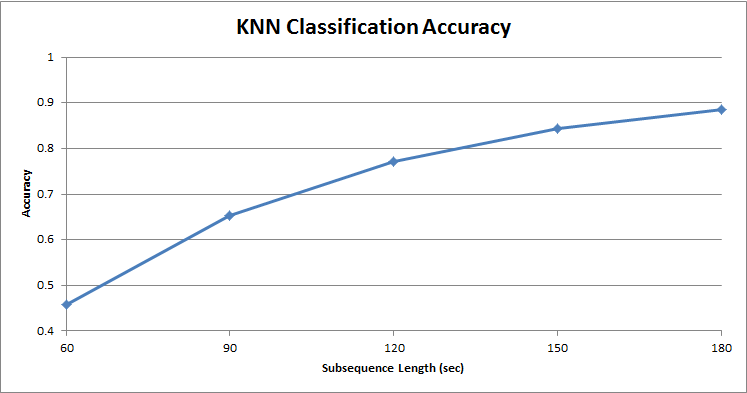
\includegraphics[scale=0.50]{Figures/experiment_knn}
\caption{KNN Classification Accuracy}
\label{fig:experiment_knn}
\vspace{-5mm}
\end{figure}